% This file is isea.tex.  It contains the formatting instructions for and acts as a template for submissions to ISEA 2015.  It is based on the ICCC  formats and instructions.  It uses the files isea.sty, isea.bst and isea.bib, the first two of which also borrow from AAAI IJCAI formats and instructions.
% Modified from ICCC.tex by B. Bogart

\documentclass[letterpaper]{article}
\usepackage{isea}
\usepackage[pdftex]{graphicx}
\usepackage{times}
\usepackage{helvet}
\usepackage{courier}
\usepackage[numbers]{natbib}
\pdfinfo{
/Title (Scaling with multiple network namespaces in a single application)
/Author (PJ Waskiewicz)}
% The file isea.sty is the style file for ISEA 2015 proceedings.
%
\title{Accelerating XDP programs using HW-based hints}
\author{PJ Waskiewicz \\ Intel \\ Hillsboro, OR, USA \\ peter.waskiewicz.jr@intel.com
\And Anjali Singhai Jain \\ Intel \\ Hillsboro, OR, USA \\ anjali.singhai@intel.com
\And Neerav Parikh \\ Intel \\ Hillsboro, OR, USA \\ neerav.parikh@intel.com
\And Parthasarathy Sarangam \\ Intel \\ Hillsboro, OR, USA \\ parthasarathy.sarangam@intel.com
\newline
\newline
}
\setcounter{secnumdepth}{0}

\begin{document} 
\maketitle
\begin{abstract}
As XDP workloads continue to evolve, they are becoming more complex.  They can parse deeper into a packet to make more complex decisions, plus they may compute more complex hashing or other CPU-intensive operations to make flow-based decisions.

This talk will focus on efforts to extend the XDP framework to pass HW-based hints that have been computed by the underlying network device.  The intent is to build a framework that is vendor agnostic, so XDP programs don't need to comprehend the underlying device they're running against.

This talk also aims to show a proposed direction for the changes in XDP, along with the proposed additional metadata structure.  It will also show benchmarks of certain XDP workloads with and without HW-based hints, highlighting the benefits of using these existing offloads.
\end{abstract}

\section{Keywords}

networking, kernel, ebpf, xdp, offloads

\section{Introduction}
XDP has already provided a giant leap forward in performance and efficiency for packet processing in many situations. To continue making progress, the eBPF and XDP infrastructure needs to utilize existing hardware offloads from a network device. This will reduce computational cycles when parsing packet headers and data, leading to more efficient eBPF and XDP programs. This progress though requires changes to the Linux kernel and surrounding eBPF infrastructure.
This paper will focus on proposed changes to eBPF and XDP for the following:
\begin{itemize}
\item Utilize HW-based offloads from a network device driver to provide hints for accelerating XDP programs
\item Share performance metrics from proof-of-concept patches highlighting the acceleration benefits of using HW hints
\item Propose future changes to the eBPF framework in LLVM, clang, and the Linux kernel, to support teaching underlying hardware which hints to provide
\item Propose additional techniques to keep XDP programs vendor-agnostic while still programming desired hints, and then consuming the hints for acceleration
\end{itemize}

\section{HW-Offloaded Hints From Device Driver} 

TBD

\begin{figure}[h]
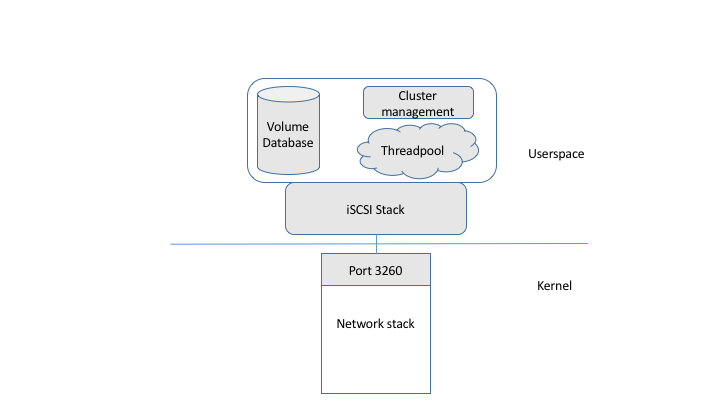
\includegraphics[width=3.31in]{standard-app-overview.png}
\caption{High-level architecture of application.}
\label{app-overview}
\end{figure}

\subsection{Initial Performance Gains}

TBD

\begin{figure}[h]
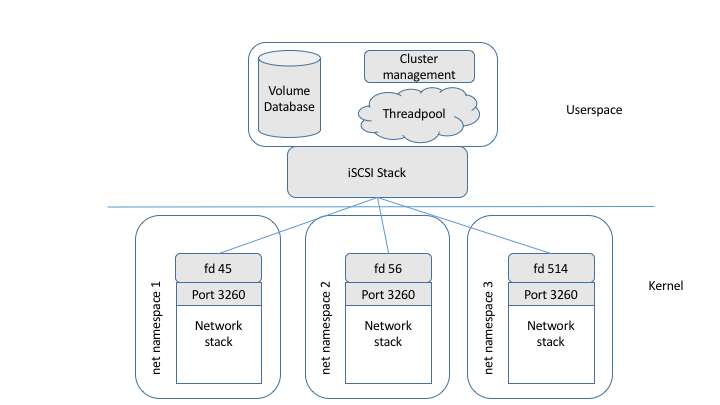
\includegraphics[width=3.31in]{multiple-namespaces-with-fd.png}
\caption{Multiple network namespaces with file descriptors.}
\label{namespace-fds}
\end{figure}

\section{Dynamic Programm of HW Hints}

TBD

\subsection{Using tc}

TBD

\subsection{Express Hints via eBPF Sections}

TBD

\subsection{XDP Per Queue}

TBD

\section{Pipelining XDP: Proposing the Future of HW Hints}

TBD

\begin{figure}[h]
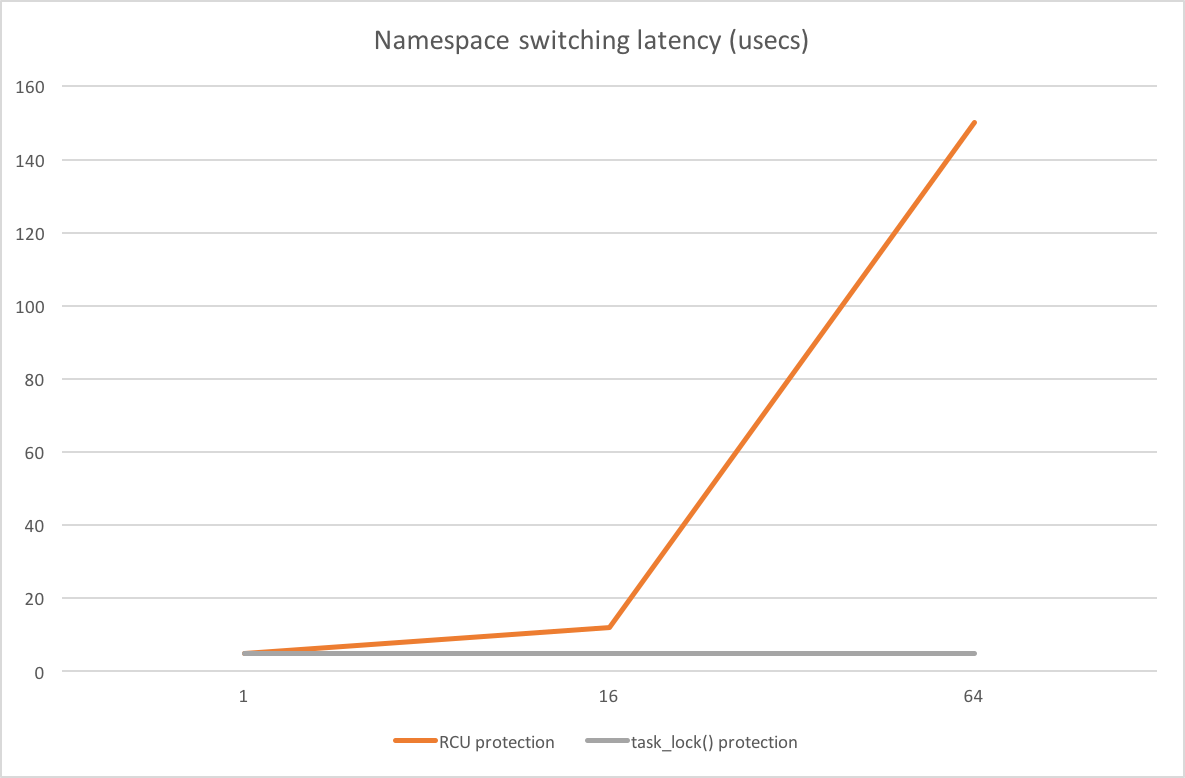
\includegraphics[width=3.31in]{close-up-latency.png}
\caption{Network namespace switching latency, close-up}
\label{close-latency}
\end{figure}

\section{Conclusion}
Utilizing smarter network device offloads is going to be crucial in maximizing the performance and efficiency of XDP programs.  As these XDP programs become more and more complex with packet processing and parsing, the natural direction is to utilize network devices as they become smarter.  However, the expression of the hints from hardware, and programming of the underlying hardware to present the hints, is something the Linux kernel network community will need to work together on to best design a sustainable and scalable model.

\section{Acknowledgments}
We would like to acknowledge the NetDev 2.2 selection committee for inviting us to submit and present this paper.

\bibliographystyle{pj-netdev-2.2}
\bibliography{pj-netdev-2.2}

\section{Author Biography}
PJ Waskiewicz is a Senior Linux Kernel Engineer in the Networking Division of Intel. He has maintained and helped create the igb, ixgbe, and i40e wired Ethernet network drivers, the initial Tx multiqueue support in the Linux kernel network stack, and added Data Center Bridging support to the Linux kernel. He also worked in Intel's Open Source Technology Center on the x86 kernel tree, enabling advanced features in the Broadwell and Skylake microarchitectures. Prior to returning to Intel, PJ was a Senior Principal Engineer at NetApp in the SolidFire division, where he was the chief Linux kernel and networking architect for the scale-out cloud storage platform.
\newline
\newline
Anjali Singhai Jain is 
\newline
\newline
Neerav Parikh is
\newline
\newline
Parthasarathy Sarangam is

\end{document}
